% Repository:  https://github.com/chiehrosswang/TRB_LaTeX_tex
%
% Transportation Research Board conference paper template
% version 4.0 Lite (updates made to be compatible in Overleaf and ShareLaTeX)
%
%
% When numbered option is activated, lines are numbered.
\documentclass[numbered]{trbunofficial}
\usepackage{graphicx}
\usepackage{booktabs}

\newread\somefile
\usepackage{xparse}
\usepackage{natbib}
\bibliographystyle{unsrtnat}
\setcitestyle{round}
% \usepackage[colorlinks=true,linkcolor=blue,citecolor=blue]{hyperref}
% For TRB version hide links
\usepackage[hidelinks]{hyperref}

% Put here what will go to headers as author
\AuthorHeaders{Anonymous, Security, and Zoolander}
\title{An Rticles Template for the Transport Research Board Annual
Meeting}

% TODO: add macros for easier formatting of \author.
\author{%
    \textbf{Alice Anonymous}\\\textit{Corresponding Author}\\
  Graduate Student\\
  Some Institute of Technology\\
  \href{mailto:alice@example.com}{\nolinkurl{alice@example.com}}\\
  \hfill\break
    \textbf{Bob Security}\\
  Assistant Professor\\
  State University\\
  \href{mailto:bob@example.com}{\nolinkurl{bob@example.com}}\\
  \hfill\break
    \textbf{Derek Zoolander}\\
  Professor\\
  Some Institute of Technology\\
  \href{mailto:derek@example.com}{\nolinkurl{derek@example.com}}\\
  \hfill\break
  }

% If necessary modify the number of words per table or figure default is set to
% 250 words per table (default defined in cls)


% If words are counted manually, put that number here. This does not include
% figures and tables. This can also be used to avoid problems with texcount
% program i.e. if one does not have it installed.
\TotalWords{684}

% Pandoc syntax highlighting
\usepackage{color}
\usepackage{fancyvrb}
\newcommand{\VerbBar}{|}
\newcommand{\VERB}{\Verb[commandchars=\\\{\}]}
\DefineVerbatimEnvironment{Highlighting}{Verbatim}{commandchars=\\\{\}}
% Add ',fontsize=\small' for more characters per line
\usepackage{framed}
\definecolor{shadecolor}{RGB}{248,248,248}
\newenvironment{Shaded}{\begin{snugshade}}{\end{snugshade}}
\newcommand{\AlertTok}[1]{\textcolor[rgb]{0.94,0.16,0.16}{#1}}
\newcommand{\AnnotationTok}[1]{\textcolor[rgb]{0.56,0.35,0.01}{\textbf{\textit{#1}}}}
\newcommand{\AttributeTok}[1]{\textcolor[rgb]{0.13,0.29,0.53}{#1}}
\newcommand{\BaseNTok}[1]{\textcolor[rgb]{0.00,0.00,0.81}{#1}}
\newcommand{\BuiltInTok}[1]{#1}
\newcommand{\CharTok}[1]{\textcolor[rgb]{0.31,0.60,0.02}{#1}}
\newcommand{\CommentTok}[1]{\textcolor[rgb]{0.56,0.35,0.01}{\textit{#1}}}
\newcommand{\CommentVarTok}[1]{\textcolor[rgb]{0.56,0.35,0.01}{\textbf{\textit{#1}}}}
\newcommand{\ConstantTok}[1]{\textcolor[rgb]{0.56,0.35,0.01}{#1}}
\newcommand{\ControlFlowTok}[1]{\textcolor[rgb]{0.13,0.29,0.53}{\textbf{#1}}}
\newcommand{\DataTypeTok}[1]{\textcolor[rgb]{0.13,0.29,0.53}{#1}}
\newcommand{\DecValTok}[1]{\textcolor[rgb]{0.00,0.00,0.81}{#1}}
\newcommand{\DocumentationTok}[1]{\textcolor[rgb]{0.56,0.35,0.01}{\textbf{\textit{#1}}}}
\newcommand{\ErrorTok}[1]{\textcolor[rgb]{0.64,0.00,0.00}{\textbf{#1}}}
\newcommand{\ExtensionTok}[1]{#1}
\newcommand{\FloatTok}[1]{\textcolor[rgb]{0.00,0.00,0.81}{#1}}
\newcommand{\FunctionTok}[1]{\textcolor[rgb]{0.13,0.29,0.53}{\textbf{#1}}}
\newcommand{\ImportTok}[1]{#1}
\newcommand{\InformationTok}[1]{\textcolor[rgb]{0.56,0.35,0.01}{\textbf{\textit{#1}}}}
\newcommand{\KeywordTok}[1]{\textcolor[rgb]{0.13,0.29,0.53}{\textbf{#1}}}
\newcommand{\NormalTok}[1]{#1}
\newcommand{\OperatorTok}[1]{\textcolor[rgb]{0.81,0.36,0.00}{\textbf{#1}}}
\newcommand{\OtherTok}[1]{\textcolor[rgb]{0.56,0.35,0.01}{#1}}
\newcommand{\PreprocessorTok}[1]{\textcolor[rgb]{0.56,0.35,0.01}{\textit{#1}}}
\newcommand{\RegionMarkerTok}[1]{#1}
\newcommand{\SpecialCharTok}[1]{\textcolor[rgb]{0.81,0.36,0.00}{\textbf{#1}}}
\newcommand{\SpecialStringTok}[1]{\textcolor[rgb]{0.31,0.60,0.02}{#1}}
\newcommand{\StringTok}[1]{\textcolor[rgb]{0.31,0.60,0.02}{#1}}
\newcommand{\VariableTok}[1]{\textcolor[rgb]{0.00,0.00,0.00}{#1}}
\newcommand{\VerbatimStringTok}[1]{\textcolor[rgb]{0.31,0.60,0.02}{#1}}
\newcommand{\WarningTok}[1]{\textcolor[rgb]{0.56,0.35,0.01}{\textbf{\textit{#1}}}}

% tightlist command for lists without linebreak
\providecommand{\tightlist}{%
  \setlength{\itemsep}{0pt}\setlength{\parskip}{0pt}}




\begin{document}
\maketitle


\section{Abstract}
The Transportation Research Board (TRB) has unique and seemingly
arbitrary requirements for manuscripts submitted for review. These
requirements make it difficult to write the manuscripts quickly, and no
existing \LaTeX~style comes close to fooling the guidelines. This
represents an initial effort at creating a template to meet the
requirements of TRB authors using \LaTeX, R, Sweave, and/or other
literate programming software.
\hfill\break%
\hfill\break%
\noindent\textit{Keywords}:  Transportation, Travel Behavior,  
\newpage

\section{Transportation Research Board Annual
Meetings}\label{transportation-research-board-annual-meetings}

TRB has greatly simplified the submissions to its system, meaning that
this template is no longer strictly required. However, there is a
typical format that most people still use by default, and this template
implements that change.

\section{Features}\label{features}

The template has a number of features that enable quick and painless
manuscript authoring.

\subsection{Mathematics}\label{mathematics}

Standard pandoc / \LaTeX math environments are available. For example,
the probability of an individual choosing alternative \(i\) in a
multinomial logit model is \begin{equation}
  P_i = \frac{exp(V_i)}{\sum_{i, j \in J}exp(V_j)} \label{eq:mnl}
\end{equation} Equations with a
\texttt{\textbackslash{}label\{eq:label\}} can be referred to later in
the text with \texttt{\textbackslash{}ref\{eq:label\}}, such as Equation
\ref{eq:mnl}.

\subsection{Title Page}\label{title-page}

The template will automatically create a title page with the authors in
the listed order. Near the bottom of the title page, TRB requires a
count of the manuscript's words and tables. The YAML header information
contains a \texttt{wordcount} key where this can be encoded. The number
of tables is counted automatically on build; a default 250 words per
table can be overriden with the \texttt{wordspertable} YAML key.

The LaTeX template available from
\url{https://github.com/chiehrosswang/TRB_LaTeX_tex} contain automatic
word counters that have not been implemented in this \texttt{rticles}
template. Authors can use the R Studio word count add-in available from
\url{https://github.com/benmarwick/wordcountaddin}.

\subsection{Page Layout}\label{page-layout}

The document has 1 inch margins as required, with the author's names in
the left heading and the page number in the right. The running header
information is set with the \texttt{runningheader} YAML key. Paragraphs
leading sections and subsections are not indented, while all subsequent
paragraphs in that section are. Section heading types are defined as
outlined by the old TRB Author's Guide.

The document is single-spaced in 12 point Times font. Times New Roman is
a proprietary font and is therefore not available by installation in
open-source software. While the differences between Times variants are
negligible, Times New Roman itself can be used in Mac OSX by compiling
under \texttt{xelatex}.

\subsection{Figure and Table
references}\label{figure-and-table-references}

The document can use standard pandoc referencing tools for in-text
citations to figures and tables. If an R code chunk outputs a figure,
the figure number can be referred to with
\texttt{\textbackslash{}@ref(fig:chunkname)} where \texttt{chunkname} is
the name of the chunk that prints the figure. For example, Figure
@ref(fig:figure-example) shows a default figure made by the R chunk
below.

\begin{Shaded}
\begin{Highlighting}[]
\CommentTok{\# Generate some sample data, then compute mean and standard deviation}
\CommentTok{\# in each group}
\NormalTok{Speed }\OtherTok{\textless{}{-}}\NormalTok{ cars}\SpecialCharTok{$}\NormalTok{speed}
\NormalTok{Distance }\OtherTok{\textless{}{-}}\NormalTok{ cars}\SpecialCharTok{$}\NormalTok{dist}
\FunctionTok{plot}\NormalTok{(Speed, Distance,}
     \AttributeTok{panel.first =} \FunctionTok{lines}\NormalTok{(stats}\SpecialCharTok{::}\FunctionTok{lowess}\NormalTok{(Speed, Distance), }\AttributeTok{lty =} \StringTok{"dashed"}\NormalTok{),}
     \AttributeTok{pch =} \DecValTok{0}\NormalTok{, }\AttributeTok{cex =} \FloatTok{1.2}\NormalTok{, }\AttributeTok{col =} \StringTok{"blue"}\NormalTok{)}
\end{Highlighting}
\end{Shaded}

\begin{figure}
\centering
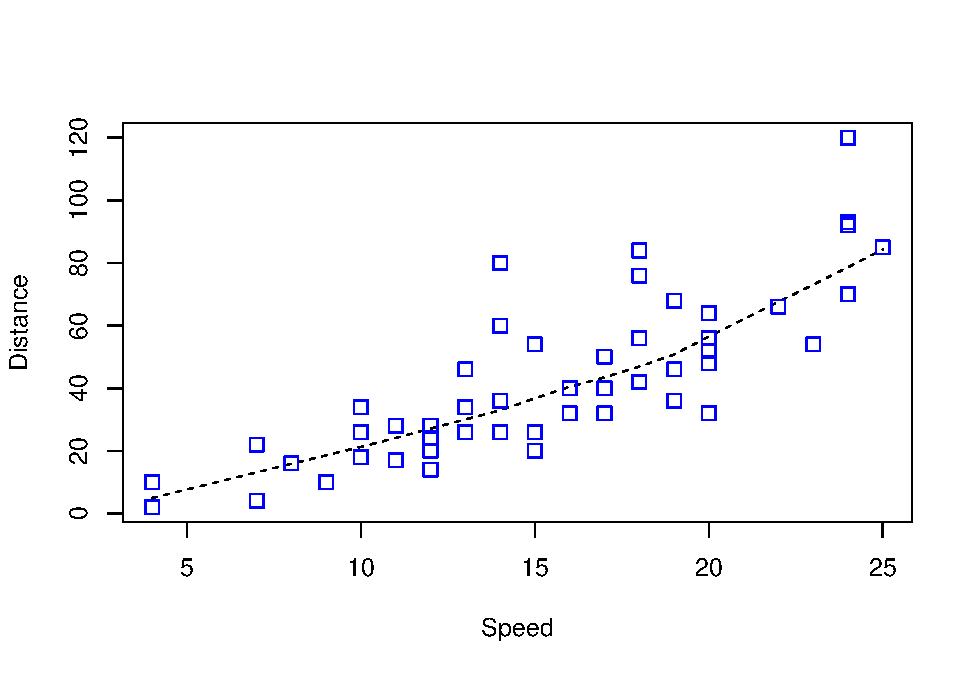
\includegraphics{grocery_store_hamilton_files/figure-latex/figure-example-1.pdf}
\caption{Generic plot.}
\end{figure}

The template setup chunk sets \texttt{echo\ =\ FALSE} for the entire
document, as printing code listings would not usually be appropriate or
needed for a TRB article. But the option is there!

The same referencing logic works for tables, with the \texttt{tab:}
prefix on the chunk name instead of \texttt{fig:} used for figures.
Table @ref(tab:table-example) has a basic table. We recommend the
\texttt{kableExtra} package for formatting publication-ready tables with
greater control than the default \texttt{knitr::kable()} function.

\begin{table}

\caption{\label{tab:table-example}Example Table}
\centering
\begin{tabular}[t]{lrrrrrr}
\toprule
  & mpg & cyl & disp & hp & drat & wt\\
\midrule
Mazda RX4 & 21.0 & 6 & 160 & 110 & 3.90 & 2.620\\
Mazda RX4 Wag & 21.0 & 6 & 160 & 110 & 3.90 & 2.875\\
Datsun 710 & 22.8 & 4 & 108 & 93 & 3.85 & 2.320\\
Hornet 4 Drive & 21.4 & 6 & 258 & 110 & 3.08 & 3.215\\
Hornet Sportabout & 18.7 & 8 & 360 & 175 & 3.15 & 3.440\\
\bottomrule
\end{tabular}
\end{table}

\subsection{Bibliography styles}\label{bibliography-styles}

TRB still wants numbered, unsorted citations beginning on a new page.
The template is configured to use \texttt{natbib} with the
\texttt{unsrtnat} citation style, with some additional logic to use
parentheses instead of brackets. The YAML key \texttt{biblio-style} will
allow the authors to select a different citation format, but this is not
recommended at the moment. Citations use the pandoc logic. Including the
reference in brackets \texttt{{[}@reference{]}} will print only the
numeric reference; e.g. \citep{Feynman1963118, Dirac1953888}. Including
the reference without brackets \texttt{@reference} will print the
authors and then the numeric reference; e.g. \citet{Feynman1963118}.

\section{Author Contribution
Statement}\label{author-contribution-statement}

The authors confirm contribution to the paper as follows: study
conception and design: A. Anonymous, D. Zoolander; data collection: B.
Security; analysis and interpretation of results: A. Anonymous, B.
Security; draft manuscript preparation: A. Anonymous. All authors
reviewed the results and approved the final version of the manuscript.

\section{Acknowledgements}\label{acknowledgements}

David Pritchard posted the original versions of this template in 2009
and updated it in 2011, soon after TRB began allowing PDF submissions.
Gregory Macfarlane and Ross Wang made adjustments to the template, and
Ross Wang now maintains the \LaTeX template at
\url{https://github.com/chiehrosswang/TRB_LaTeX_tex}. Gregory Macfarlane
created the \texttt{rticles} template in 2021.

\newpage
\renewcommand\refname{References}
\bibliography{mybibfile.bib}


\end{document}
